
%---------------------------------------%
% Packages arranged by : Tsz Timmy Chan %
%                 Date : May 26th, 2019 % 
%---------------------------------------%

\documentclass{TC}
\usepackage{TCcommon}

\title{TITLE HERE}	% Work Title Here.
\author{Tsz Timmy Chan}	% YOUR NAME HERE 

\usepackage[notes]{TCheader}
\usepackage{TCexamtitle}

\usepackage{setspace}
\linespread{1.5}

%\renewcommand{\benediction}{" " - }
%\renewcommand{\quoteoftheday}{" " \\ - }

\begin{document}



Reading start to get a bit philosophical \parencite{bredo_philosophies_2006}.
	\begin{itemize}
		\item The author gave four ways of "getting to the bottom" of an idea :
			\begin{enumerate}
			\item "Method of tenacity": just hold your opinion really hard, which fails when your opponent is equally tenacious;
			\item "Method of authority": appeal to authority in a particular community, which fails when the authorities are not in agreement;
			\item "Method of a priori reasoning": finding underlying beliefs or assumptions that are common, which fails when the beliefs come from differently epistemologies,
			\item "Method of experiment": different epistemologies should be adopted as hypothetical and fallible, and tested in terms of their consequences. 			\end{enumerate}
		\item The author discussed the distinctions between \gls{externalist} and \gls{internalist} views, and the third, \gls{interactionism}, which is in between the two mentioned here.
		\item The thoughts leading up to post-positivism, post-modernism and critical theory.
		\item \Gls{externalist} thoughts $\implies$ \gls{empiricism} $\implies$ \gls{classicalpositivism} and  \gls{logicalpositivism}. Critiques of positivism that follow in succession of this line of \gls{externalist} school of thought thought are together taken as \gls{postpositivism}---though those who subscribe to postpositivism tend to still believe a model of research based on natural sciences, with the goals of searching for universal laws. This is in the left branch of \autoref{fig:green_philosophies}.
		\item Kantian rationalism is a critique of previous \gls{rationalism} on that it focuses too much on the mind (like Descartes, Spinoza and Leibniz) and also denounces the approach of \gls{empiricism} as focusing too little on the mind. 
		\item A tool that arose during the time of the development of these Romantic responses to Enlightenment \gls{empiricism} is \gls{hermeneutics}, which Dilthey (1833-1911) suggests that this methodological foundation provides a framework for cultural sciences distinct from natural sciences.
		\item \Gls{internalist} thoughts $\implies$ \gls{subjectiveidealism} $\implies$ \gls{structuralism}. Critiques of these eventually lead to \gls{postmodernism}; even structuralism has a given, where $\exists$ a structure at all. This is in the middle branch of \autoref{fig:green_philosophies}.
		\item \Gls{dialectic}al/Transactional Relation $\implies$ \gls{absoluteidealism} $\implies$ \gls{dialecticalmaterialism} $\implies$ \gls{criticaltheory} This is in the right-most branch of \autoref{fig:green_philosophies}.
		\item \Gls{criticaltheory} arose as a response to \gls{instrumentalrationality}
		\item And finally, standing on its own is\gls{pragmatism}, where local progress is possible without a notion of progress towards ultimate ends or directions. Truth is a matter of an idea's usefulness in guiding action. 
	\end{itemize}
	
	\begin{itemize}[(???)]
		\item What did the author mean when they said "Newton's explanation of planetary motion based on the law of gravitation really is correct, then empiricism \emph{must} be wrong because it cannot not account for such universal and necessary generalizations."?
	\end{itemize}
	\begin{itemize}[(!!!)]
	\item The text is indeed dense, but written in a way that is not conducive for reading by non-philosophers. In particular, the author chose to use words before they are well defined, and I believe the author did not do a good job at defining subjective idealism. 
	
	\item Similarly, transcendentalism was in the title of a section without once being defined.
	\item "knowing is primarily for the sake of action, and action changes what is known"
	\end{itemize}

\begin{figure}[H]
\centering
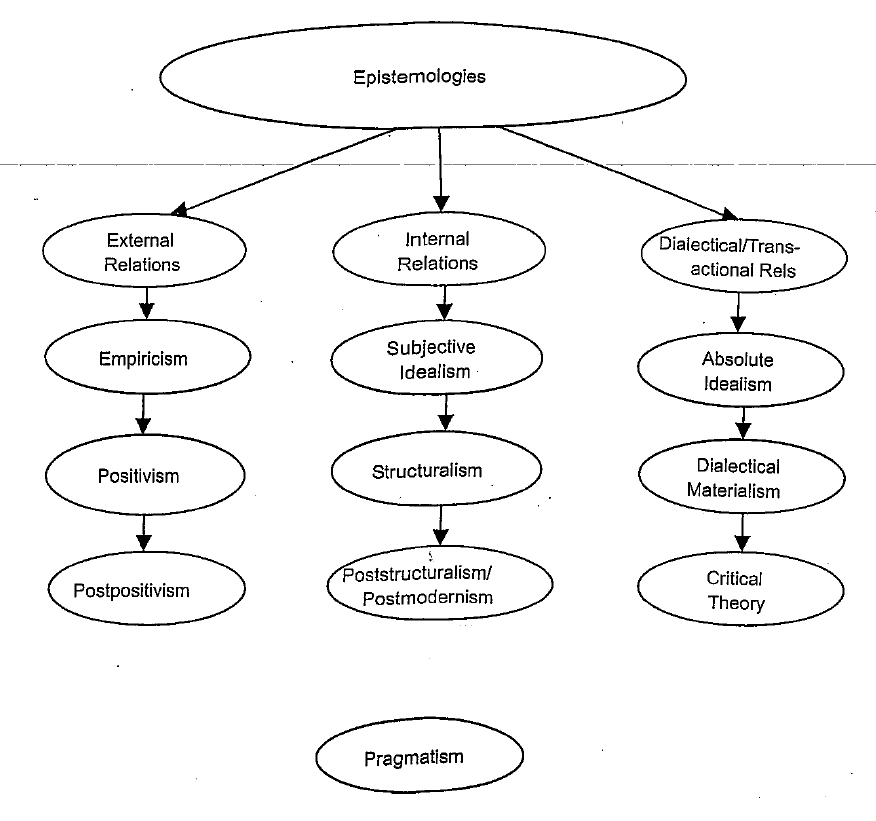
\includegraphics[width=.7\textwidth]{bredo_philosophies.png}
\caption{Arrangement of philosophies \parencite{green_philosophies_2006}}
\label{fig:green_philosophies}
\end{figure}
	
	\end{document}
